\startchapter{Fast Estimation of Power Quality}
\label{chap:PQEstimation}
\small
In this chapter, we propose a maximum-entropy (MaxEnt) based approach to estimating power quality in smart microgrid. Compared to other existing methods such as Monte Carlo Expectation Maximization (MCEM), the MaxEnt based approach is much faster.

\normalsize
\section{Introduction}
Power quality largely impacts the reliability and energy saving of power networks. Poor power quality such as voltage sags may lead to power outage and service interruptions. Service unavailability caused by power losses is a serious problem for many companies and organizations, e.g., it may result in a significant revenue loss for Internet service providers or even loss of lives in hospitals. To improve the reliability of power networks, organizations and large companies (e.g., Google data centers) adopt smart microgrid, and closely monitor the power quality in different segments of the microgrid.

Monitoring power quality, however, is not an easy task. Since the power measurement devices~\cite{fluke_meter}\cite{schneider_meter} (termed as smart meters in this thesis) are expensive, it is financially impractical to monitor every segment of a power network. The overhead of interconnecting these power meters and developing the power management system further increases the cost. In addition, in many cases direct monitoring of power quality is difficult, e.g., it is hard to install smart meters after power lines were sealed in hard-to-reach areas in a building. In general, we need to tackle the following challenge: based on a limited small number of monitored points in a power network, \textit{how can we effectively estimate the power quality of other unmonitored segments of the network?} 

We propose to use a Maximum-Entropy (MaxEnt)~\cite{maxent} approach to power quality estimation. The basic idea of MaxEnt is that out of all probability distributions consistent with a given set of constraints (i.e., the known measure values in our case), we should choose the one that has the maximum uncertainty to be the estimated power quality values. Intuitively, the principle of MaxEnt implies that we should make use of all the information that is given and avoid making (biased) assumptions about information that is not available. We model the problem of estimating power quality in such a way where we can effectively get the benefit of MaxEnt approach to correctly estimate the power quality values at links where we do not have any measuring device installed. We solve the formulated MaxEnt problem and validate its effectiveness and efficiency with a simulated microgrid system.

\section{Related Work}
According to the IEEE Gold Book~\cite{goldbook}, the industry practices for electric power quality in networks focus on measures such as reliability, availability, and Mean Time Between Failures (MTBF). While it is known~\cite{iti_curve} that lifetime and performance of electrical components are dependent on power quality, none of the measures defined in the IEEE Gold Book accounts for power quality. Moreover, these measures serve as theoretical values for comparisons and are not intended to work in real environment (with varying temperature, humidity, load, and power quality) as predictive tools for networks. Further, the ITI curve report illustrates the relationship between power quality and the likelihood of damage to electric components. While considering the importance of both the magnitude and duration of power quality events in isolation, it does not consider its cumulative effects over time.

The EM algorithm is one of the most widely-used algorithms for estimation and has been applied in a variety of research areas.
 In~\cite{catherine_pri}, the authors investigate the power of EM algorithm in the estimation of microgrid reliability. Although effective, the EM algorithm needs a long time to converge. We are thus motivated to find faster algorithms in power quality estimation for smart microgrid.

\begin{landscape}
\begin{figure}[!p]
    \centering
    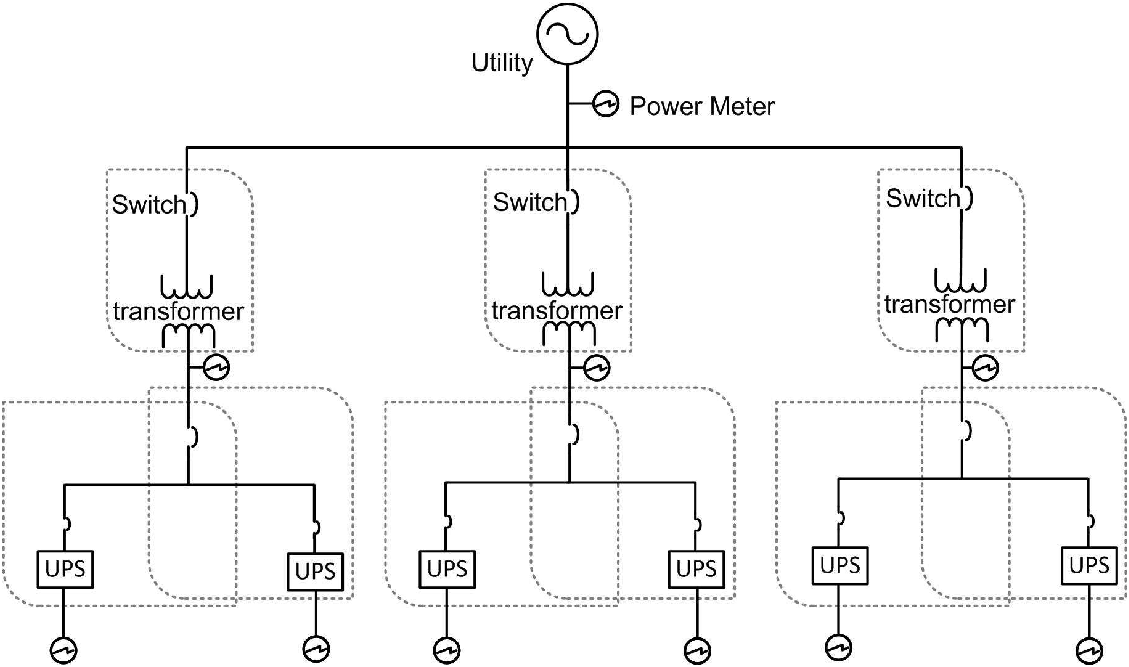
\includegraphics[width=1.2\textwidth]{subnetview}
    \vspace{0.5cm}    
    \caption{View of the power grid network under consideration. Subnets (within dotted lines) are formulated based on the positions of the power meters.}
    \vspace{1.5cm}
    \label{fig:subnetview}
\end{figure}
\end{landscape}

The measurement and monitoring of power quality are a vital part of today's smart grid. To classify power quality, a label is assigned to a power quality event, based on the feature of the event, e.g., the magnitude and duration of a voltage sage or swell. Typically, the power quality index, also known as System Average RMS Variation Frequency Index (SARFI), is reported as a count of the number of times the magnitude and duration fall below a threshold, standardized by the IEEE standard 1159-2009~\cite{IEEE09_1159}.


\section{Problem Formulation}
Figure~\ref{fig:subnetview} shows a view of a power grid where there are different types of electrical devices connected to each other via power links. The smart meters are also installed on selected links. Moreover, every type of device has a power quality function which may be unknown. We want to estimate all the power quality functions based on the power quality values available on selected links where smart meters are installed. We divide the power grid network into small subnets where in every subnet we have two smart meters, i.e., one at the input as the first node and one at the output as the last node of the subnet as shown in Figure~\ref{fig:subnetview}.

Now, we consider every subnet as a single node which we call a black-box. For every black-box, we know the power quality values at the input as well as at the output. Based on this known power quality information, we calculate the power quality transition function by using some sample readings from the smart meters attached to both sides of every black-box. Figure~\ref{fig:subnet} shows a sample subnet as a single node. We represent the calculated power quality function $f(s)$  of subnet $s$ as a matrix as follows:

\vspace{1cm}
\begin{equation}
f(s) = \left[\begin{array}{cccc} p_{c_1 \mid c_1}^{(s)} & p_{c_2 \mid c_1}^{(s)} & \cdots & p_{c_n \mid c_1}^{(s)}\\
p_{c_1 \mid c_2}^{(s)} & p_{c_2 \mid c_2}^{(s)} & \cdots & p_{c_n \mid c_2}^{(s)}\\
\vdots & \vdots& \ddots & \vdots\\
p_{c_1 \mid c_n}^{(s)} & p_{c_2 \mid c_n}^{(s)} & \cdots & p_{c_n \mid c_n}^{(s)}
\end{array}\right],
%\label{eqn:pqf}
\end{equation}
\vspace{1cm}

\noindent
where $p_{c_y  \mid c_x}^{(s)}$ is the probability that the input quality $c_x$ is received as $c_y$ at the output of the subnet $s$. Moreover, the value of $p_{c_y  \mid c_x}^{(s)}$ can be easily calculated by measuring power quality values at the input and output smart meters of the subnet. Note that every row in the above matrix must sum to $1$.

\begin{figure*}[!p]
\centering
	\subfloat[A subnet containing 2 devices.]{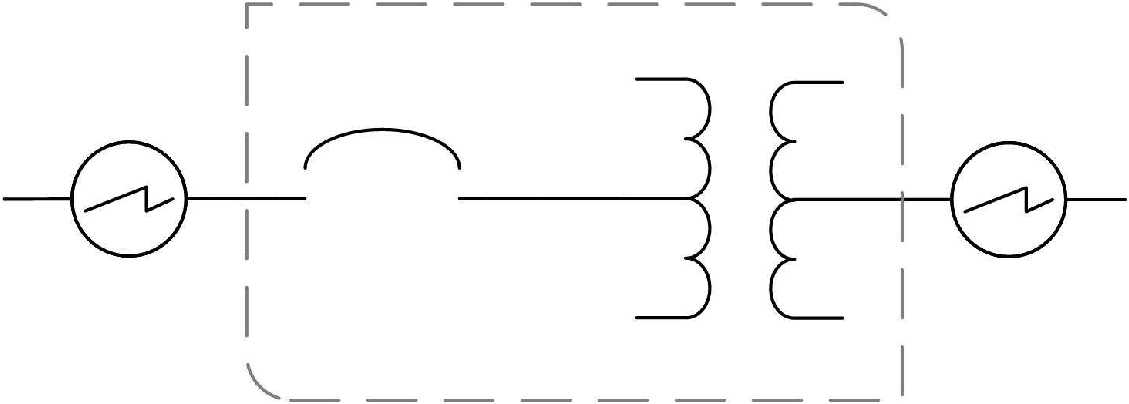
\includegraphics[width=0.7\textwidth]{subnet_1}}\\ \vspace{1cm}
	\subfloat[Subnet as a single power transition matrix.]{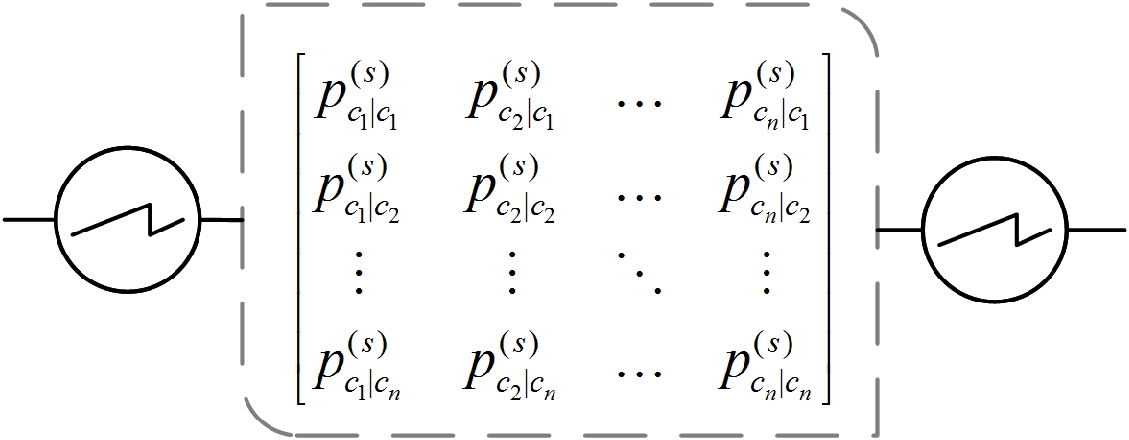
\includegraphics[width=0.7\textwidth]{subnet_2}}\\ \vspace{1cm}
	\subfloat[Power transition matrix of each device $d_j$.]{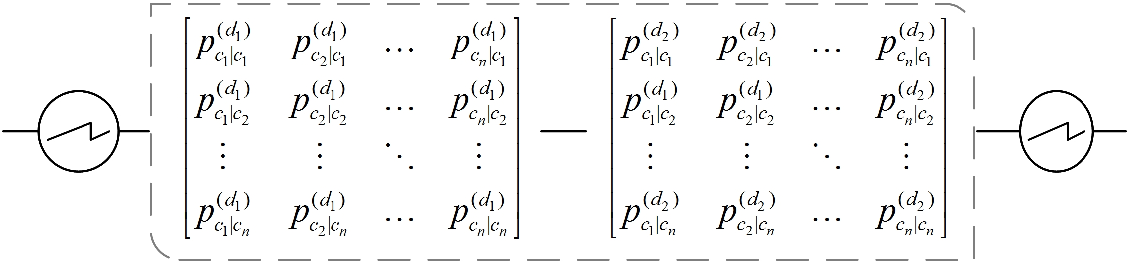
\includegraphics[width=0.98\textwidth]{subnet_3}} \\\vspace{0.5cm}
\caption{The power transition matrix $f(s)$ of a subnet $s$ as a product of the power transition matrices of individual devices.} \label{fig:subnet}
\end{figure*}

Figure~\ref{fig:subnet}(a) shows a subnet containing two devices. The power quality transition function (as a matrix) of the subnet is shown inside the black-box in Figure~\ref{fig:subnet}(b). Our objective is to correctly estimate the transition functions of every device $d_j$ in the subnet. These unknown functions are shown as matrices in Figure~\ref{fig:subnet}(c).

In order to estimate the reliability of every device in the network, we need to estimate the power quality function $f(d_j)$ for each device $d_j$ based on the quality function $f(s)$ of the subnet. It is clear that

\vspace{0.5cm}
\begin{equation}
f(s) = \prod_{j} f(d_j),
\end{equation}
\vspace{0.5cm}

\noindent
which implies that


\begin{equation}
\left[\begin{array}{ccc}
p_{c_1  \mid c_1}^{(s)} & \cdots & p_{c_n  \mid c_1}^{(s)}\\
\vdots & \ddots & \vdots\\
p_{c_1  \mid c_n}^{(s)} & \cdots & p_{c_n  \mid c_n}^{(s)}
\end{array}\right]= \prod_j { \left[\begin{array}{ccc}
p_{c_1 \mid c_1}^{(d_j)} & \cdots & p_{c_n  \mid c_1}^{(d_j)}\\
\vdots & \ddots & \vdots\\
p_{c_1 \mid c_n}^{(d_j)} & \cdots & p_{c_n \mid c_n}^{(d_j)}\end{array}\right]}
\label{eqn:product}
\end{equation}
\vspace{1cm}

Our objective is to estimate $p_{c_y \mid c_x}^{(d_j)}$ (probability that power quality $c_x$ will be mapped to power quality $c_y$ at each device $d_j$). We use the data estimation techniques to solve Eq.~(\ref{eqn:product}).

\vspace{0.5cm}
\section{Power Quality Estimation using Entropy Maximization}
\label{sec:formulation}
Modeling the microgrids as data-driven networks helps us utilize the best available data estimation techniques to solve the power quality estimation problem. One of the most popular and widely-used data estimation techniques is EM algorithm. In a recent study~\cite{catherine_pri}, the authors successfully applied the EM algorithm to power quality estimation in microgrid. Although effective, the EM algorithm took a long time to converge. In this work, we propose to use a MaxEnt approach to estimating the power quality of unmonitored segments of the grid. Before we formulate the power quality estimation problem as a MaxEnt problem, first we give a short description of EM and MaxEnt algorithms.

\vspace{0.5cm}
\subsection{The Expectation Maximization (EM) Algorithm} EM is a general approach to iterative computation of maximum-likelihood estimates when the observations can be viewed as incomplete data. Since each of the iteration of the algorithm consists of an expectation step followed by a maximization step, the algorithm is named as the EM algorithm. The successive iterations always increase the likelihood and the algorithm converges at a stationary point.

\vspace{0.5cm}
\subsection{The Maximum Entropy (MaxEnt) Algorithm} MaxEnt solves convex optimization problems of the form,
\[\mathrm{\mathbf{maximize}}~g(\vec{x}) = - \sum_{i=1}^n x_i \log x_i \]
\[\mathrm{subject~to~} \mathbf{A}\vec{x} \leq \mathbf{c},~ \mathbf{B}\vec{x} = \mathbf{1},\]

where $\vec{x}\in \mathbb{R}^n$ is the optimization variable, $A \in \mathbb{R}^{m \times n}$, and $B \in \mathbb{R}^{m \times n}$ are problem parameters;  and \textbf{1} is a vector with all 1's.

\vspace{0.5cm}
\subsection{Our MaxEnt-based Estimation of Power Quality} We model the power quality estimation problem as the MaxEnt problem to accurately estimate the power quality transition functions $f(d_j)$ with acceptable efficiency. Obviously, there are multiple possible power quality functions $f(d_j)$ which are consistent with Eq.~(\ref{eqn:product}). We consider only those solutions which not only satisfy Eq.~(\ref{eqn:product}) but are consistent with other design constraints, for instance: 1) every row in the matrix $f(d_j)$ must sum to $1$ (or at least very close to $1$); and 2) $p_{c_y \mid c_x}^{(d_j)}$ must not be negative. Other possible constraints are discussed later in this section.

The basic idea of using MaxEnt here is that out of all possible quality functions (probability distributions) consistent with the design constraints, we choose the one with maximum uncertainty. Intuitively, the principle of MaxEnt implies that we should make use of all the information (design constraints) that is available and avoid making (biased) assumptions about information that is not available. Our objective function becomes,
\begin{equation} \label{objective}
\mathrm{\mathbf{maximize}}~g = -\sum_{j, ~x, ~y} p_{c_y \mid c_x}^{(d_j)} \log p_{c_y \mid c_x}^{(d_j)}
\end{equation}

subject to following constraints:
\begin{enumerate}\itemsep0.5em
\item All components of the estimated functions $f(d_j)$ must not be negative, that is,
\begin{equation}
 p_{c_y \mid c_x}^{(d_j)} \geq 0
\end{equation}
\item Every row of $f(d_j)$ sum to 1. To allow negligible rounding errors, we introduce a small rounding error factor ($\varepsilon_1$) to be tolerated, i.e., 
\begin{equation}
	\abs{ 1 - \sum_y  p_{c_y \mid c_x}^{(d_j)} } \leq \varepsilon_1, \ \ \forall x \label{cons2}
\end{equation}

\item The estimated functions $f(d_j)$ satisfy the condition $\prod_j f(d_j) = f(s)$. One may relax the condition by a small approximation error factor ($\varepsilon_2$) to adjust the rounding errors. This adjustment is necessary when we are interested in a close approximation of $f(s)$. This condition becomes,
\begin{equation}
\abs{ f(s) - \prod_j f(d_j) } \leq \varepsilon_2. \label{con3}
\end{equation}

Note that we slightly abuse the notation for simplicity. We use $-$ above to represent an element wise minus of two matrices and $\abs{.}$ to change the values in the matrix to their absolute values. In addition, the symbol $\leq$ means all values in the left matrix is no larger than $\varepsilon_2$.

\item Every component of the estimated function $f(d_j)$ must not vary from its corresponding component of the ``true" transition function $\acute{f}(d_j)$ by a factor $\varepsilon_3$, i.e.,
\begin{equation}
\abs{ f(d_j) - \acute{f}(d_j)} \leq \varepsilon_3 \label{con4}
\end{equation}
The meanings of the notations are the same as above.
\end{enumerate}

\begin{remark}
In practice, we do not know $\acute{f}(d_j)$. To avoid this problem, we can \textit{initially} set $\acute{f}(d_j)$ as the transition function of the same type of device, which may be obtained via its specification or historical data of monitored devices of the same type. As time goes, this initial setting of $\acute{f}(d_j)$ should be updated with the optimal estimation function, i.e., $\acute{f}(d_j)$ is set to equal $f(d_j)$, and the updated $\acute{f}(d_j)$ is used for the next round of estimation. Such iterative updates capture the transition function of the (unmonitored) device, which may change over time.
\end{remark}

\begin{remark}
Someone may argue that our solution may be biased toward the last constraint (i.e., Eq.~\ref{con4}). By ignoring the last constraint, we get many solutions consistent to the first three constraints and our objective function chooses the one having maximum uncertainty. Here, if we do not use constraint 4 (Eq. ~\ref{con4}), we will be ignoring some known information about the transition functions of the unmonitored devices which may result in compromising the accuracy of the estimated transition functions. Further, in some rare cases, the last constraint may not be feasible when an obtained transition functions ($f(d_j)$) is different by an amount greater than $\varepsilon_3$ . In that case, we may ignore the last constraint or increase the value of $\varepsilon_3$.
\end{remark}

\begin{remark}
It is worth noting that the objective function~(\ref{objective}) is a non-Shannon measure, because $\sum_{j, ~x, ~y} p_{c_y \mid c_x}^{(d_j)} = \sum_{j}\sum_{x}\sum_{y} p_{c_y \mid c_x}^{(d_j)} >1$. Nevertheless, by maximizing this non-Shannon measure, we obtain a good estimation of transition functions as demonstrated in our experimental evaluation. This is not by coincidence, since the objective function could be considered as the sum of several Shannon entropy functions (i.e., Given $x$ and $j$, $\sum_{y} p_{c_y \mid c_x}^{(d_j)}\log p_{c_y \mid c_x}^{(d_j)}$ is a Shannon entropy measure). In our case, we treat each entropy function with the same weight. If we have more knowledge regarding the distribution of input power quality events, assigning different weights to different entropy functions may lead to better estimation. We leave this exploration as future work.  \end{remark}

\begin{remark}
This work focuses on a centralized processing and as such we assume that there exists an underlying communication system to support data collection to a central point. The implementation of this communication system is beyond the scope of this work. Further, the real-time issues of the monitoring and communication systems such as the data sampling and communication delay are ignored in the work.
\end{remark}

\begin{table}[!p]
\centering  \caption{Transition functions of various electrical components obtained using our latent feature model.} \label{tbl:dev_trans}
\renewcommand{\tabcolsep}{0.3 cm}
\renewcommand*{\arraystretch}{1.1}
\subfloat[Bus]{
\begin{tabular}{|m{0.3cm}m{0.3cm}|m{1cm}m{1cm}m{1cm}m{1cm}m{0.5cm}|}
\hline
& & \multicolumn{5}{c|}{\textbf{Output PQ}} \\
& & $c_1$ & $c_2$ & $c_3$ & $c_4$ & $c_5$ \\
\hline
\multirow{5}{*}{\rotatebox{90}{\textbf{Input PQ}}}& $c_1$ &  0.9	&	0.1	&	0	&	0	& 0 \\
& $c_2$ & 0	&	0.9	&	0.1	&	0	& 0\\
& $c_3$ & 0	&	0	&	0.9	&	0.1	& 0\\
& $c_4$ & 0	&	0	&	0	&	0.9	& 0.1\\
& $c_5$ & 0	&	0	&	0	&	0	& 1\\
\hline
\end{tabular}
}

\subfloat[Switch]{
\begin{tabular}{|m{0.3cm}m{0.3cm}|m{1cm}m{1cm}m{1cm}m{1cm}m{0.5cm}|}
\hline
& & \multicolumn{5}{c|}{\textbf{Output PQ}} \\
& & $c_1$ & $c_2$ & $c_3$ & $c_4$ & $c_5$ \\
\hline
\multirow{5}{*}{\rotatebox{90}{\textbf{Input PQ}}}& $c_1$ &  0.7	&	0.1	&	0.1	&	0.05	& 0.05 \\
& $c_2$ & 0 	&	0.7	&	0.1	&	0.1		& 0.1\\
& $c_3$ & 0	&	0	&	0.7	&	0.2	& 0.1\\
& $c_4$ & 0	&	0	&	0	&	0.7	& 0.3\\
& $c_5$ & 0	&	0	&	0	&	0	& 1\\
\hline
\end{tabular}
}

\subfloat[Transformer]{
\begin{tabular}{|m{0.3cm}m{0.3cm}|m{1cm}m{1cm}m{1cm}m{1cm}m{0.5cm}|}
\hline
& & \multicolumn{5}{c|}{\textbf{Output PQ}} \\
& & $c_1$ & $c_2$ & $c_3$ & $c_4$ & $c_5$ \\
\hline
\multirow{5}{*}{\rotatebox{90}{\textbf{Input PQ}}}& $c_1$ &  0.85	&	0.15	&	0	&	0	& 0 \\
& $c_2$ & 0.15	&	0.7	&	0.15	&	0	& 0 \\
& $c_3$ & 0	&	0.15	&	0.7	&	0.15	& 0 \\
& $c_4$ & 0	&	0	&	0.15	&	0.7	& 0.15 \\
& $c_5$ & 0	&	0	&	0	&	0	& 1 \\
\hline
\end{tabular}
}

\subfloat[UPS]{
\begin{tabular}{|m{0.3cm}m{0.3cm}|m{1cm}m{1cm}m{1cm}m{1cm}m{0.5cm}|}
\hline
& & \multicolumn{5}{c|}{\textbf{Output PQ}} \\
& & $c_1$ & $c_2$ & $c_3$ & $c_4$ & $c_5$ \\
\hline
\multirow{5}{*}{\rotatebox{90}{\textbf{Input PQ}}}& $c_1$ &  1	&	0	&	0	&	0	& 0 \\
& $c_2$ & 0.8	&	0.2	&	0	&	0	& 0 \\
& $c_3$ & 0.8	&	0	&	0.2	&	0	& 0 \\
& $c_4$ & 0.8	&	0	&	0	&	0.2	& 0 \\
& $c_5$ & 0.8	&	0	&	0	&	0	& 0.2 \\
\hline
\end{tabular}
}
\end{table}

\begin{figure}[!p]
\centering \vspace{2cm}
	\subfloat{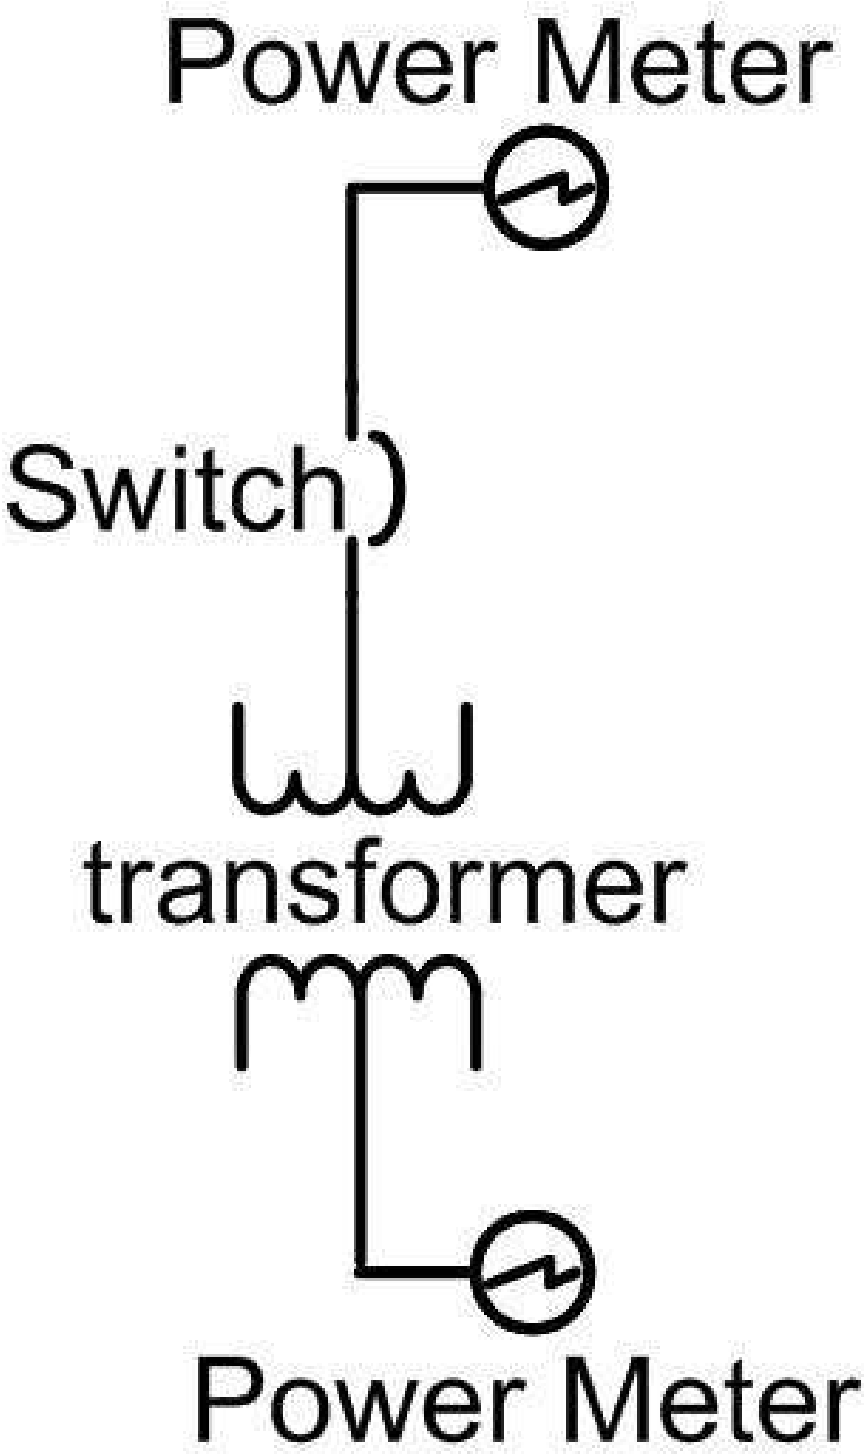
\includegraphics[width=0.20\columnwidth]{s1}}\\ \vspace{1cm}
	\subfloat{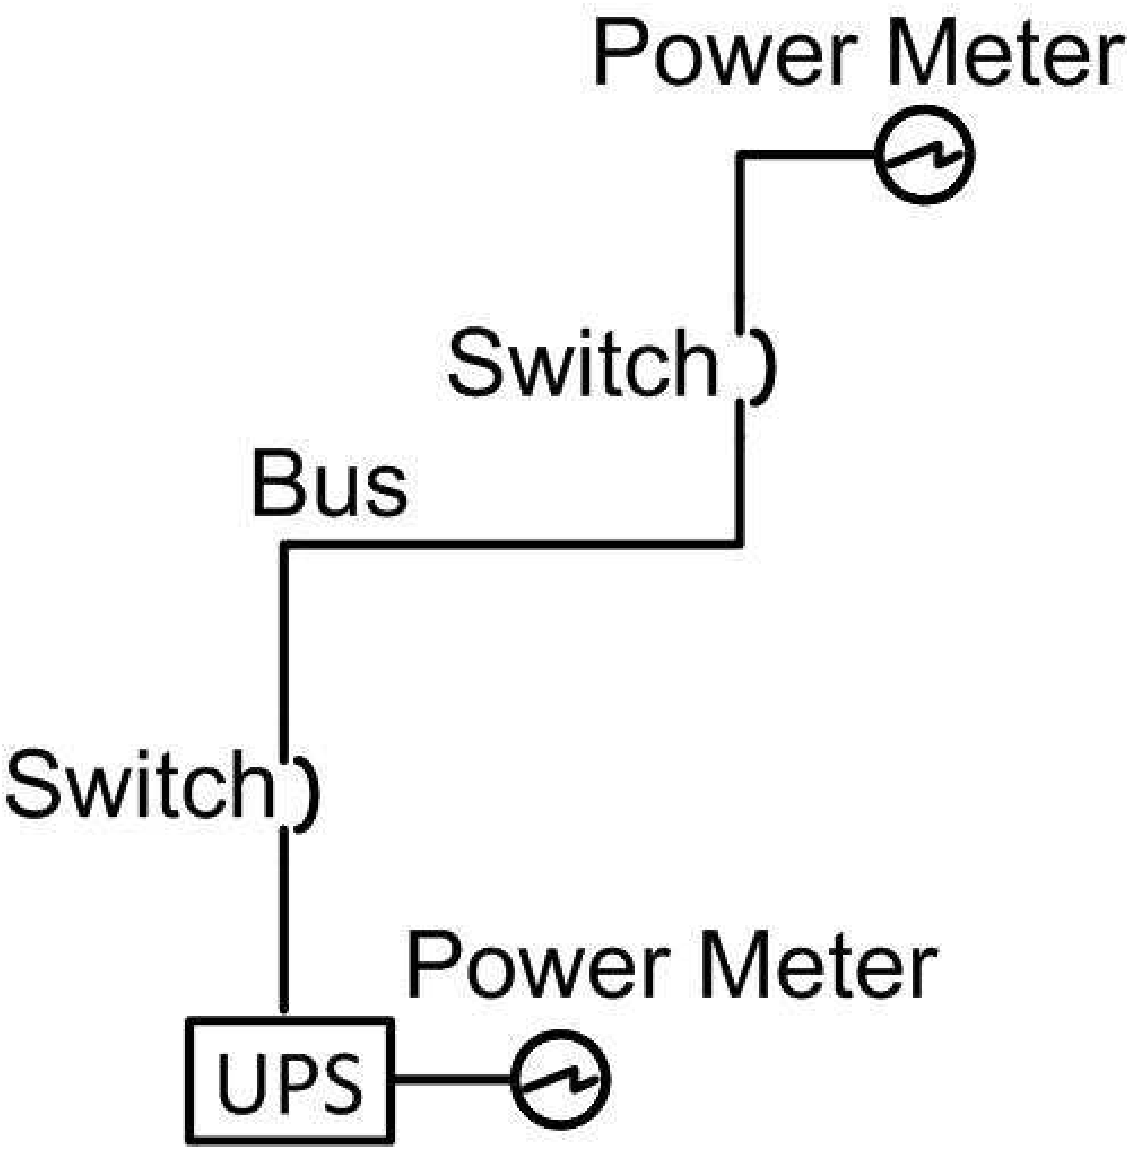
\includegraphics[width=0.33\columnwidth]{s2}}
	\vspace{0.5cm}
\caption{Two different kinds of subnets. The one at the left side containing two devices (switch, transformer) and the one shown at the right side containing four devices (switch, bus, switch, and UPS).} \label{fig:twosubnets} \vspace{2cm}
\end{figure}

\begin{table}[!p]
\vspace{2cm}
\renewcommand{\tabcolsep}{0.2 cm}
\renewcommand*{\arraystretch}{2}
\centering \caption{Convergence time (in seconds) comparison of MaxEnt vs EM algorithms.}
\begin{tabular}{|c|c|c|c|c|c|}
 \hline \multicolumn{2}{|c|}{\multirow{2}{*}{}} & \multirow{2}{*}{\textbf{MaxEnt}} & \multicolumn{3}{c|}{\textbf{Expectation Maximization (EM)}}\\
\cline{4-6}
\multicolumn{2}{|c|}{} & & Iteration 5 & Iteration 10 & Iteration 15\\
\hline
\multirow{2}{*}{\textbf{Subnet size}} & 2 & 2.16 & 40.3 & 117.7 & 402.6\\
\cline{2-6}
& 4 & 3.42 & 118.32 & 366.9 & 981.01\\
\hline
\end{tabular}
\label{tbl:eval_t}
\end{table}


\begin{table}[!p]
\renewcommand{\tabcolsep}{0.2 cm}
\renewcommand*{\arraystretch}{2}
\centering \caption{Mean squared error comparison of MaxEnt vs EM algorithms.}
\begin{tabular}{|c|c|c|c|c|c|}
 \hline \multicolumn{2}{|c|}{\multirow{2}{*}{}} & \multirow{2}{*}{\textbf{MaxEnt}} & \multicolumn{3}{c|}{\textbf{Expectation Maximization (EM)}}\\
\cline{4-6}
\multicolumn{2}{|c|}{} & & Iteration 5 & Iteration 10 & Iteration 15\\
\hline
\multirow{2}{*}{\textbf{Subnet size}} & 2 & 0.00020 & 0.00017 & 0.00013 & 0.00010\\
\cline{2-6}
& 4 & 0.00030 & 0.00025 & 0.00019 & 0.00014\\
\hline
\end{tabular}
\vspace{4cm}
\label{tbl:eval_mse}
\end{table}

\section{Performance Evaluation}
\label{sec:evaluation}
We implement the proposed objective function and simulate a power microgrid using MATLAB. The view of the simulated network is shown in Figure~\ref{fig:gridNetwork} where only several network segments are monitored using smart meters. Our objective is to estimate the power quality values on network segment where no smart meter is installed. We use the same transition functions as in~\cite{catherine_pri} as the ground truth. These power quality transition functions of various electrical components (switch, bus, ups, and transformer etc) in the smart grid are shown in Table~\ref{tbl:dev_trans}.

We use non-linear constrained optimization algorithm named Sequential Quadratic Programming (SQP) to estimate the unknown power quality functions. Inputs to the algorithm are the known power quality functions for each subnet $f(s)$, error tolerance factors $\varepsilon_1 = \varepsilon_2 = 0.01$, and $ \varepsilon_3 = 0.05$. The error tolerance is small enough for practical applications. The power quality matrix of each subnet is the product of the power transition functions (shown in Table~\ref{tbl:dev_trans}) of the devices in that subnet. The simulated microgrid consists of subnets of two different sizes; one contain two devices (switch and a transformer) while the other containing four devices (switch, bus, switch, and UPS). Both of these subnets are shown in Figure~\ref{fig:twosubnets}. The power transition matrices of each subnet are calculated by multiplying the ground truth matrices of devices used in the corresponding subnet. Further, the simulation was performed on a desktop computer having Intel Dual-Core-i7 3.4 GHz processor with $4$ GB physical memory.

Table~\ref{tbl:eval_t} shows the convergence time comparison of both the EM and MaxEnt based solutions to power quality estimation. It can be seen that the convergence time of MaxEnt is much faster as compared to that of EM algorithm. The convergence time is exponentially increasing for the EM algorithm with the network size. For a real-time estimation, the convergence time is more important and the EM based solution is not feasible to operate in real-time given its huge convergence delays. We measure the estimation accuracy using Mean Squared Error (MSE), which is a statistical measure quantifying the difference between values implied by an estimator and the true values of the quantity being estimated. The results are shown in Table~\ref{tbl:eval_mse}. From the results, we can see that both the methods give very close estimations of the power quality transition functions, i.e., the difference between the estimated and corresponding ground truth functions is negligible.

%\begin{figure}[!t]
%    \centering
%    \includegraphics[width=0.9\columnwidth]{mse}
%    \caption{Mean Squared Error comparison of MaxEnt vs EM algorithms.}
%    \label{fig:mse}
%\end{figure}

\section{Conclusion}
Reliability of power grid networks is critically important in today's life.  Smart meters play an important role in estimating reliability of power networks but they are expensive devices and it is financially infeasible to install them on every link between devices in the power grid network. We propose a MaxEnt based model that accurately estimates power quality transition functions on unmonitored network segments. The experimental results show that 1) our MaxEnt based solution is much faster than the existing EM based solution to power quality estimation; and 2) the proposed solution accurately estimates the power transition functions. Finally, the MaxEnt based model opens a new scope of methods to quantitatively measure and solve the reliability problems in smart grid.